% Essential Formatting

\documentclass[12pt]{article}
\usepackage{epsfig,amsmath,amsthm,amssymb}
\usepackage[english]{babel}
\usepackage{subfigure}
\usepackage[questions, answersheet]{urmathtest}[2001/05/12]
%\usepackage[answersheet]{urmathtest}[2001/05/12]
%\usepackage[answers]{urmathtest}[2001/05/12]


% For use with pdflatex
% \pdfpagewidth\paperwidth
% \pdfpageheight\paperheight

% Basic User Defs

\def\ds{\displaystyle}

\newcommand{\ansbox}[1]
{\work{
  \pos\hfill \framebox[#1][l]{ANSWER:\rule[-.3in]{0in}{.7in}}
}{}}

\newcommand{\ansrectangle}
{\work{
  \pos\hfill \framebox[6in][l]{ANSWER:\rule[-.3in]{0in}{.7in}}
}{}}


% Beginning of the Document

\begin{document}
\examtitle{LINEAR REGRESSION MODELS W4315}{HOMEWORK 4}{10/08/2009}
 \begin{center}
  Instructor: Frank Wood 
 \end{center}
%%\studentinfo
\instructions{
  %\textbf{Circle your Instructor's Name along with the Lecture Time:}



  \begin{itemize}
  \item
    \textbf{Please show all your work.
            You may use back pages if necessary.}
  %\item
   % \textbf{Please put your \underline{simplified}
   %         final answers in the spaces provided.}
  \end{itemize}
}
\finishfirstpage

% Problems Start Here % ----------------------------------------------------- %


\problem{50} {\footnote[1]{This is
problem 3.4 in `Applied Linear Regression Models(4th edition)' by
Kutner etc.} 
 Refer to \textbf{Copier maintenance} Problem 1.20.\\
 a. Prepare a dot plot for the number of copiers serviced $X_i$. What information is provided by this plot? Are there any outlying cases with respect to this variable?\\
 b. The cases are given in time order. Prepare a time plot for the number of copiers serviced. What does your plot show?\\
 d. Prepare residual plots of $e_i$ versus $\hat{Y_i}$ and $e_i$ versus $X_i$ on separate graphs. Do these plots provide the same information? What departures from regression model (2.1) can be studied from these plots? State your findings. And the model (2.1) is as follows:\\
 \begin{center}
 $Y_i=\beta_0+\beta_1 X_i+\epsilon_i$\\
 \end{center}
 where:\\
 \begin{center}
 $\beta_0$ and $\beta_1$ are parameters\\
 $X_i$ are known constants\\
 $\epsilon_i$ are independent $N(0,\sigma^2)$
 \end{center}
 e. Prepare a normal probability plot of the residuals. Also obtain the coefficient of correlation between the ordered residuals and their expected values under normality. DOes the normality assumption appear to be tenable here? Use table B.6 and $\alpha=.10$.\\
 f. Prepare a time plot of the residuals to ascertain whether the error terms are correlated over time. What is your conclusion?\\
 h. Information is given below on two variables not included in the regression model, namely, mean operational age of copiers serviced on the call($X_2$, in months) and years of experience of the service person making the call($X_3$). Plot the residuals against $X_2$ and $X_3$ on separate graphs to ascertain whether the model can be improved by including either or both of these variables. What do you conclude?\\
N.B. 1. If you need any software for this problem, do not use the
embedded linear regression commands, say, 'regress' in MATLAB is not allowed.
2. If you are using software, please attach the code at the back of your
handed-in homework instead of mixing codes with the results.
3. You don't have to hand in part c and h of this problem. 
}
 { \vfill
  \answer
} { (a) Continuing the code from last homework with the same
notation, the R code to draw the plot is: boxplot(x), which is illustrated in figure 1.
\begin{figure}[h!]
  \caption{3.3a box plot of the ACT scores}
  \centering
    \includegraphics[scale=.4]{a.png}
\end{figure}
There doesn't seem to be anything noteworthy about the ACT scores other than it seems rather symmetric with no apparent outliers. The median seems to lie exactly in the middle of the range and the IQR.
Because the data size is 120, we can be fairly certain that the distribution is symmetrical.\\
(b) The R code is: dotchart(y-y.hat) which gives the dot plot of
residuals:
\begin{figure}[h!]
  \caption{3.3b dot plot of the residuals}
  \centering
     \includegraphics[scale=.4]{b.png}
\end{figure}
It shows roughly the distribution of the error terms. It appears to be centered around 0 and does look normal. However, there are a couple of outliers.\\
(c) The R code is:\\
\begin{center}
plot(y.hat,y-y.hat,xlab="fitted Y values",ylab="residuals")
\end{center}
which give the residual plot as:
\begin{figure}[h!]
  \caption{3.3c residual plot}
  \centering
     \includegraphics[scale=.4]{c.png}
\end{figure}
There are a few residuals that depart quite distantly from the
regression model as seen in the plot. But in general, the residuals
are scattered evenly about the model without a pattern, which is a
good thing for
setting up the linear regression model.\\
(d) The R code to draw a qq-plot is "qqnorm" or "qqplot", who have
different parameters. You are suggested to go check the detail using
R built-in help system.
Here we can use:\\
$qqnorm(res)$\\
$qqline(res,col=2)$\\
directly to draw the qqplot as follows:
\begin{figure}[h!]
  \caption{3.3d qqplot to test normality assumption of the model}
  \centering
     \includegraphics[scale=.4]{d.png}
\end{figure}
As for the correlation between the sorted residuals and expected value under normality assumption,
we can use the following R code:\\
$sort\_res <- sort(res,index.return=TRUE)\$x$\\
$index <- sort(res,index.return=TRUE)\$ix$\\
$expected\_under\_normal <- sqrt(MSE)*pnorm((c(1:n)-.375)/(n+.25))$\\
$cor(sort\_res,expected\_under\_normal)$ $\to$ this is the test statistics r\\
In this specific setting, the formulation of the hypothesis is:\\
$H_0: Normality assumption holds \leftrightarrow H_1: Normality assumption fails$\\
Then we get the correlation between the two is around .97. Refer to Table B.6 and we can find that $.97<.98$, so we reject $H_0$ which means that the normality assumption doesn't hold here. This
keeps sync with conclusion that we can get from the qqplot, since from it, we can see that the dots do not all align up on one straight line. But also notice that the skewness is not severe and the
test statistics is not far smaller than the criteria. So normality assumption may not hold here, but the violation is not very significant.\\
(d)Conduct the Brown-Forsythe test:\\
$res.1 <- res[x<26]$\\
$res.2 <- res[x>=26]$\\
$n1 <- length(res.1)$\\
$n2 <- length(res.2)$\\
$med.1 <- median(res.1)$\\
$med.2 <- median(res.2)$\\
$d1 <- abs(res.1-med.1)$\\
$d2 <- abs(res.2-med.2)$\\
$s <- sqrt((sum((d1-mean(d1))^2)+sum((d2-mean(d2))^2))/(n-2))$\\
$t.BF <- (mean(d1)-mean(d2))/s/(sqrt(1/n1+1/n2))$\\
$qt(.995,n-2)$\\
The decision rule is that if $|t.BF| < t(.995,118)$, then we accept the $H_0$, otherwise we reject it. Here we have t.BF to be -0.896, so we accept the assumption that error terms have equal variances, or at least
the error variance does not vary with the level of X. It does not contradict the conclusion we arrived at (c).\\
(f)
The R code is:\\
$x2 <- data[,3]$\\
$x3 <- data[,4]$\\
$plot(x2,res,xlab="intelligence test score",ylab="residuals")$\\
$plot(x3,res,xlab="high school class rank percentile",ylab="residuals")$\\
The residual plots are:(Please refer to the last page.)
\begin{figure}[ht]
  \centering
  \subfigure[3.3f plot of residuals against $X_2$]{
  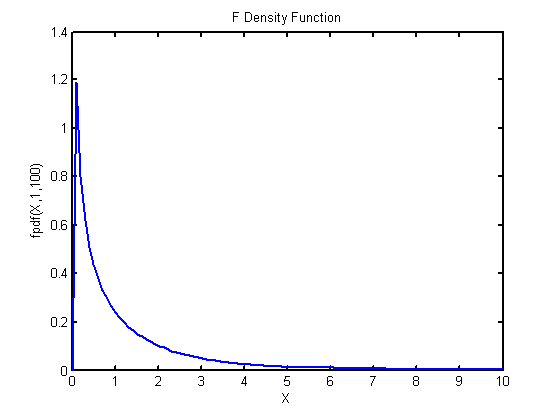
\includegraphics[scale=.4]{f1.png}}
  \subfigure[3.3f plot of residuals against $X_3$]{
  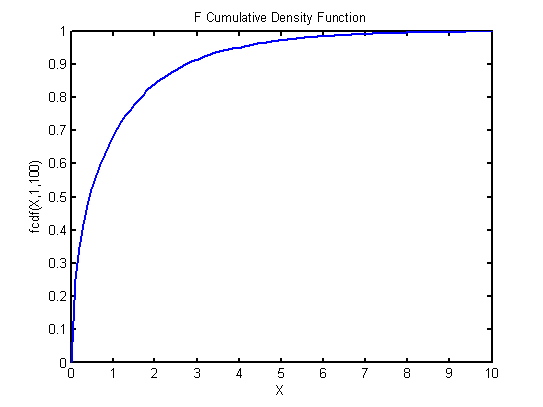
\includegraphics[scale=.4]{f2.png}}
\end{figure}
From the graphs we can see there is a transparent linear trend between the residuals and X2, but no obvious trend between residuals and X3. So we should include X2 into
our model, and proceed to further investigation into the case concerning X3.\\
 }

\problem{25} {\footnote[2]{This is
problem 3.19 in `Applied Linear Regression Models(4th edition)' by
Kutner etc.} 
 A student fitted a linear regression function for a class assignment. The student plotted the residuals $e_i$ against $Y_i$ and found a positive relation. When the residuals were plotted against the fitted values $\hat{Y_i}$, the student found no relation. How could this difference arise? Which is the more meaningful plot?
} { \vfill
  \answer
} { In either cases, the residuals represent the distance from the
Y's to the fitted Y's. If there is no violation of the assumptions,
there should be apparent pattern when plotting residuals again the
fitted Y values, which is more meaningful when carrying out residual
analysis. As for plotting residuals against observed Y's, it should
always manifest positive relations between the two, so it's not
sensible. You can explain this from two perspectives. One is by
intuition: for large Y's, it is more likely that the values depart
from the regression line(especially if the line is pretty flat, and
the data are more spread out), and for small Y values, it's more
likely that they're somewhere around the regression line, thus have
a less significant residual.  Another way to explain the positive
correlation comes from the decomposition of the Y:\\
$\hat{e}=Y-\hat{Y}$, so we have $Y=\hat{e}+\hat{Y}$. Since $\hat(Y)$
and $\hat(e)$ are independent, we have that the covariance between
$\hat(e)$ and $Y$ is always positive, even when the assumption is
violated. In this sense, the residual plot against fitted Y is more
meaningful, actually it is the most classic residual plot that we
usually use. }

\problem{25} {\footnote[3]{This is
problem 3.20 in `Applied Linear Regression Models(4th edition)' by
Kutner etc.} 
 If the error terms in a regression model are independent $N(0,\sigma^2)$, what can be said about the error terms after transformation $X'=1/X$ is used? Is the situation the same after transformation $Y'=1/Y$ is used?
} { \vfill
  \answer
} { If the transformation is exerted only on X, then the error terms
remain normally distributed, however, the mean will shift--this is
because X is not taken as random variables in the regression
setting, so if only X is transformed, the model's distribution of
course is not going to change.\\
Nevertheless, if Y is reversed, then the error term's distribution
will change in the way that it will not even follow a normal
distribution. This is simply because the reverse of a normally
distributed random variable will not still follow normal
distribution. So when taking transformations, we should be careful
about the inference made after fitting the model, since the
distribution may be different than which we carry forward the
classic inference.}


% Problems End Here % ------------------------------------------------------- %

\problemsdone
\end{document}

% End of the Document
